% Options for packages loaded elsewhere
\PassOptionsToPackage{unicode}{hyperref}
\PassOptionsToPackage{hyphens}{url}
\PassOptionsToPackage{dvipsnames,svgnames,x11names}{xcolor}
%
\documentclass[
  letterpaper,
  DIV=11,
  numbers=noendperiod]{scrreprt}

\usepackage{amsmath,amssymb}
\usepackage{iftex}
\ifPDFTeX
  \usepackage[T1]{fontenc}
  \usepackage[utf8]{inputenc}
  \usepackage{textcomp} % provide euro and other symbols
\else % if luatex or xetex
  \usepackage{unicode-math}
  \defaultfontfeatures{Scale=MatchLowercase}
  \defaultfontfeatures[\rmfamily]{Ligatures=TeX,Scale=1}
\fi
\usepackage{lmodern}
\ifPDFTeX\else  
    % xetex/luatex font selection
\fi
% Use upquote if available, for straight quotes in verbatim environments
\IfFileExists{upquote.sty}{\usepackage{upquote}}{}
\IfFileExists{microtype.sty}{% use microtype if available
  \usepackage[]{microtype}
  \UseMicrotypeSet[protrusion]{basicmath} % disable protrusion for tt fonts
}{}
\makeatletter
\@ifundefined{KOMAClassName}{% if non-KOMA class
  \IfFileExists{parskip.sty}{%
    \usepackage{parskip}
  }{% else
    \setlength{\parindent}{0pt}
    \setlength{\parskip}{6pt plus 2pt minus 1pt}}
}{% if KOMA class
  \KOMAoptions{parskip=half}}
\makeatother
\usepackage{xcolor}
\setlength{\emergencystretch}{3em} % prevent overfull lines
\setcounter{secnumdepth}{-\maxdimen} % remove section numbering
% Make \paragraph and \subparagraph free-standing
\ifx\paragraph\undefined\else
  \let\oldparagraph\paragraph
  \renewcommand{\paragraph}[1]{\oldparagraph{#1}\mbox{}}
\fi
\ifx\subparagraph\undefined\else
  \let\oldsubparagraph\subparagraph
  \renewcommand{\subparagraph}[1]{\oldsubparagraph{#1}\mbox{}}
\fi


\providecommand{\tightlist}{%
  \setlength{\itemsep}{0pt}\setlength{\parskip}{0pt}}\usepackage{longtable,booktabs,array}
\usepackage{calc} % for calculating minipage widths
% Correct order of tables after \paragraph or \subparagraph
\usepackage{etoolbox}
\makeatletter
\patchcmd\longtable{\par}{\if@noskipsec\mbox{}\fi\par}{}{}
\makeatother
% Allow footnotes in longtable head/foot
\IfFileExists{footnotehyper.sty}{\usepackage{footnotehyper}}{\usepackage{footnote}}
\makesavenoteenv{longtable}
\usepackage{graphicx}
\makeatletter
\def\maxwidth{\ifdim\Gin@nat@width>\linewidth\linewidth\else\Gin@nat@width\fi}
\def\maxheight{\ifdim\Gin@nat@height>\textheight\textheight\else\Gin@nat@height\fi}
\makeatother
% Scale images if necessary, so that they will not overflow the page
% margins by default, and it is still possible to overwrite the defaults
% using explicit options in \includegraphics[width, height, ...]{}
\setkeys{Gin}{width=\maxwidth,height=\maxheight,keepaspectratio}
% Set default figure placement to htbp
\makeatletter
\def\fps@figure{htbp}
\makeatother

\KOMAoption{captions}{tableheading}
\makeatletter
\@ifpackageloaded{caption}{}{\usepackage{caption}}
\AtBeginDocument{%
\ifdefined\contentsname
  \renewcommand*\contentsname{Table of contents}
\else
  \newcommand\contentsname{Table of contents}
\fi
\ifdefined\listfigurename
  \renewcommand*\listfigurename{List of Figures}
\else
  \newcommand\listfigurename{List of Figures}
\fi
\ifdefined\listtablename
  \renewcommand*\listtablename{List of Tables}
\else
  \newcommand\listtablename{List of Tables}
\fi
\ifdefined\figurename
  \renewcommand*\figurename{Figure}
\else
  \newcommand\figurename{Figure}
\fi
\ifdefined\tablename
  \renewcommand*\tablename{Table}
\else
  \newcommand\tablename{Table}
\fi
}
\@ifpackageloaded{float}{}{\usepackage{float}}
\floatstyle{ruled}
\@ifundefined{c@chapter}{\newfloat{codelisting}{h}{lop}}{\newfloat{codelisting}{h}{lop}[chapter]}
\floatname{codelisting}{Listing}
\newcommand*\listoflistings{\listof{codelisting}{List of Listings}}
\makeatother
\makeatletter
\makeatother
\makeatletter
\@ifpackageloaded{caption}{}{\usepackage{caption}}
\@ifpackageloaded{subcaption}{}{\usepackage{subcaption}}
\makeatother
\ifLuaTeX
  \usepackage{selnolig}  % disable illegal ligatures
\fi
\IfFileExists{bookmark.sty}{\usepackage{bookmark}}{\usepackage{hyperref}}
\IfFileExists{xurl.sty}{\usepackage{xurl}}{} % add URL line breaks if available
\urlstyle{same} % disable monospaced font for URLs
\hypersetup{
  pdftitle={Electoral Votes Apportionment},
  pdfauthor={Yi Wang},
  colorlinks=true,
  linkcolor={blue},
  filecolor={Maroon},
  citecolor={Blue},
  urlcolor={Blue},
  pdfcreator={LaTeX via pandoc}}

\title{Electoral Votes Apportionment}
\author{Yi Wang}
\date{2024-10-07}

\begin{document}
\maketitle
\section{To win US presidency: 270 electoral
votes}\label{to-win-us-presidency-270-electoral-votes}

\begin{itemize}
\item
  Total electoral votes (electors): 538
\item
  Senators: \(50 \cdot 2 + 435\) (Congress) \(+ 3\) (Washington D.C.,
  not considered as a state)
\end{itemize}

\section{How the 435 congressional seats are
distributed?}\label{how-the-435-congressional-seats-are-distributed}

\begin{itemize}
\item
  By population of each state
\item
  Principle: equal representation (votes per seat)
\item
  Each state must have at least one Congressional seat (50)
\item
  Remaining \(435-50= 385\).
\end{itemize}

\section{How to solve the problem}\label{how-to-solve-the-problem}

Calculation of a Congressional apportionment requires three factors

\begin{itemize}
\tightlist
\item
  the apportionment population of each state,
\item
  the number of representatives to be allocated among the states,
\item
  and a method to use for the calculation.
\end{itemize}

\section{What populationt to use?}\label{what-populationt-to-use}

Article 1, Section 2, of the Constitution sets the basis: Decennial
census of population (1790-present, except 1920), with the provision
that each state must have at least one representative.

\section{Ideally: Hare Quota (votes per
seat)}\label{ideally-hare-quota-votes-per-seat}

\[
\text{votes per seat }(\lambda)= \frac{\text{Total US population }(P)}{435}\,.
\] \[
\begin{aligned}
\textbf{entilted} \text{ seats of each state }(t^*_i)&= \frac{\text{Total state population }(P_i)}{\lambda}\,\\
\sum_{i=1}^n{t^*_i}&=1\,.
\end{aligned}
\]

\textbf{Problem}: \(t^*_i\) is in general \textbf{fractional}. Not
practical.

\section{Method of Fixed Ratio}\label{method-of-fixed-ratio}

\begin{itemize}
\tightlist
\item
  Rounding up
\item
  Rounding down
\item
  Standard rounding (round 5 up and 4 down)
\end{itemize}

\textbf{New problem}: variable seats (too many or too few)

\begin{itemize}
\item
  1787-1790 (first enumeration): 65 set by the Constitution
\item
  1790-1830 (Jefferson method: fixed ratio with rounding down):
  resulting 105 seats.
\item
  1840 (Webster method): fixed ratio with standard rounding.
\end{itemize}

\section{Fixed House Size}\label{fixed-house-size}

\begin{itemize}
\tightlist
\item
  1911: House size was fixed at 433 with provision for the addition of
  one seat each for Arizona and New Mexico when they became states (U.S.
  Statutes at Large, 37 Stat 13, 14 (1911))
\item
  The House size, 435 members, has been unchanged since, except for a
  temporary increase to 437 at the time of admission of Alaska and
  Hawaii as states (following the 1950 census until the 1960 census).
\end{itemize}

\section{Mathematical Formulation}\label{mathematical-formulation}

Given \((t_1,t_2,\cdots, t_k)\), find a vector of non-negative integers
\((n_1,n_2,\cdots, n_k)\), such that \[
\begin{aligned}
\sum_{i=1}^k{t^*_i}&=1\\
\sum_{i=1}^k n_i &=h\,.
\end{aligned}
\] \[\text{minimize expectated } \textbf{ errors or seat bias}\,.\]
e.g.~favoring smaller parties, or large parties, etc.

\section{Quota Rule}\label{quota-rule}

The \emph{quota rule} describes a desired property of proportional
apportionment methods. It says that the number of seats allocated to a
party should be equal to their entitlement plus or minus one.

\section{Apportionment Paradoxes}\label{apportionment-paradoxes}

\begin{itemize}
\item
  \textbf{Alabama Paradox} A state could receive fewer representatives
  if the size of the House increased.
\item
  \textbf{Population paradox} \(A\) grows at a faster rate than \(B\),
  i.e., \({ A/B}\) increases, then \({ A}\) should not lose a seat while
  \({B}\) gains a seat.
\item
  \textbf{No-show paradox} A particularly severe variant, where voting
  for a party causes it to lose seats.
\item
  \textbf{Spoiler effect}: a spoiler is a losing candidate who affects
  the results of an election simply by participating, causing voters to
  change their opinions.
\end{itemize}

\section{How to solve the problem with fixed house size
(1850-1900)?}\label{how-to-solve-the-problem-with-fixed-house-size-1850-1900}

\begin{enumerate}
\def\labelenumi{\arabic{enumi}.}
\tightlist
\item
  \textbf{Largest remainder method}(Hamilton/Vinton method) first assign
  integral seats to each state, then assign the remaining seat one at a
  time with the largest remainder.
\end{enumerate}

\begin{itemize}
\tightlist
\item
  \textbf{Advantage}: Meet the quota rule
\item
  \textbf{Problem}: sbj. population, Alabama, no-show paradox.
\item
  Had Congress used Webster or Hamilton's method (as it had since 1840),
  the 1876 election would have gone to Tilden instead of Hayes.
\end{itemize}

\section{How to solve the problem with fixed house size (1910,
1930)}\label{how-to-solve-the-problem-with-fixed-house-size-1910-1930}

\begin{enumerate}
\def\labelenumi{\arabic{enumi}.}
\setcounter{enumi}{1}
\tightlist
\item
  (1910, 1930) \textbf{Webster method with a pre-selected fixed ratio}:
  The ratio was selected (trial-and-error) so that the result would be
  the predetermined size of the House of Representatives.
\end{enumerate}

\section{How to solve the problem with fixed house
size}\label{how-to-solve-the-problem-with-fixed-house-size}

\begin{enumerate}
\def\labelenumi{\arabic{enumi}.}
\setcounter{enumi}{2}
\tightlist
\item
  \textbf{Highest vote average (votes per seat)}: Starting from 0 for
  each state, assign a seat one a time to the state that has the highest
  vote \textbf{average} per seat.
\end{enumerate}

Average by dividing \(P_i\) by

\begin{itemize}
\tightlist
\item
  \(n\)
\item
  \((n+1)\)\\
\item
  between \(n\) and \((n+1)\) (continuity correction)? which one?
\end{itemize}

\section{Highest Vote Average (votes per seat) Method (Divisor
Method)}\label{highest-vote-average-votes-per-seat-method-divisor-method}

\begin{itemize}
\tightlist
\item
  Adam (divided by the current seats \(n\); rounding up)
\item
  Jefferson/D'Hondt (divided by \((n+1)\); rounding down) favors large
  parties. ``\textbf{ghosts of departed representatives}''
\item
  Webster/Saine-Lagne (divided by \(n+\frac{1}{2}\), standard rounding:
  unbiased in terms of expected seat bias).
\item
  Huntington-Hill (Method of equal proportions) (divided by
  \(\sqrt{n\cdot(n+1})\), Geometric rounding): unbiased in terms of
  relative percentage error, adopted by \textbf{U.S. Congress} (US code
  Title 2) in 1941 following the census of 1940.
\end{itemize}

\section{Comparison and historical
anecdotes}\label{comparison-and-historical-anecdotes}

\begin{itemize}
\item
  Huntington-Hill's method and Webster's method very similar;
\item
  when first used, differed only in whether assigned a single seat to
  Michigan or Arkansas.
\item
  Following the 1990 census, two lawsuits concerning apportionment
  issues were filed in federal courts. The \textbf{U.S. Supreme Court}
  held that the \textbf{method of equal proportions was constitutional};
\item
  US Department of Commerce v. Montana 112 S.Ct. 1415 (1992) and
  Franklin v. Massachusetts 112 S.Ct. 2767 (1992).
\end{itemize}

\section{Propoerties of Divisor Methods (Highest Vote
Averge)}\label{propoerties-of-divisor-methods-highest-vote-averge}

\begin{itemize}
\tightlist
\item
  Monotoniciy: voting for a party can never cause it to lose seats
  (No-show paradox)
\item
  House Monononiciy: Increasing the number of seats should not case a
  state to lose a seat (Alabama Paradox)
\item
  Min-Max inequality: It is impossible to lower the highest vote average
  by reassigning a sear from one party to another. \[
  \max \left\{\frac{\text{votes[party]}}{\text{post(seats[party])}}\right\} \le \min \left\{\frac{\text{votes[party]}}{\text{post(seats[party])}+1}\right\}
  \]
\end{itemize}

\section{Huntington-Hill Method( Equal Proportions Method):
1940-}\label{huntington-hill-method-equal-proportions-method-1940-}

\begin{itemize}
\item
  Every party begins with 0 seats. Then, at each iteration, allocate a
  seat to the party with the highest vote average (votes per seat)
  divided by \(\sqrt{n(n+1)}\).
\item
  Minimizes the relative difference in the number of constituents
  represented by each legislator. In other words, no transfer of a seat
  from one state to another can reduce the percent error in
  representation for both states.
\item
  Conceptually, this method rounds to the integer that has the smallest
  relative (percent) difference.
\end{itemize}

\section{Huntington-Hill Method
(Details)}\label{huntington-hill-method-details}

Compute a \emph{priority value} \[
A_n=\frac{P_i}{\sqrt{n(n+1})},\quad n: \text{seats before allocaiton}\,.
\]

\begin{itemize}
\tightlist
\item
  \(51\)st \(\rightarrow\) \textbf{California} with the largest
  \(A_1\).\\
\item
  \(52\)nd \(\rightarrow\) \textbf{Texas}, because its \(A_1>A_n\) of
  any other state.
\item
  \(53\)st \(\rightarrow\) \textbf{California} because its \(A_2>A_n\)
  of any other state.
\item
  \(54\)th \(\rightarrow\) \textbf{New York} because its \(A_1>A_n\) of
  any other state at this point.
\end{itemize}

\section{Example}\label{example}

\begin{itemize}
\tightlist
\item
  \(P_A=100\,000\), \(P_B=80\,000\), \(P_C=30\,000\),
  \(P_A+P_B+P_C=210\,000\).
\item
  Total number of seats \(=8\).
\item
  Ideal seats =\(\frac{P_i}{P_A+P_B+P_C}\cdot 8\).
  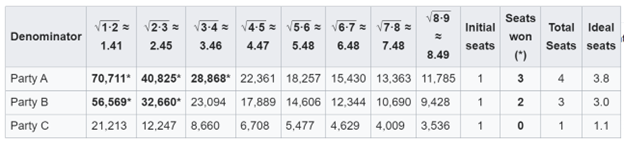
\includegraphics[width=10.41667in,height=\textheight]{images/Huntington-Hill.png}
\end{itemize}

\section{Ghost of Departed
Representatives}\label{ghost-of-departed-representatives}

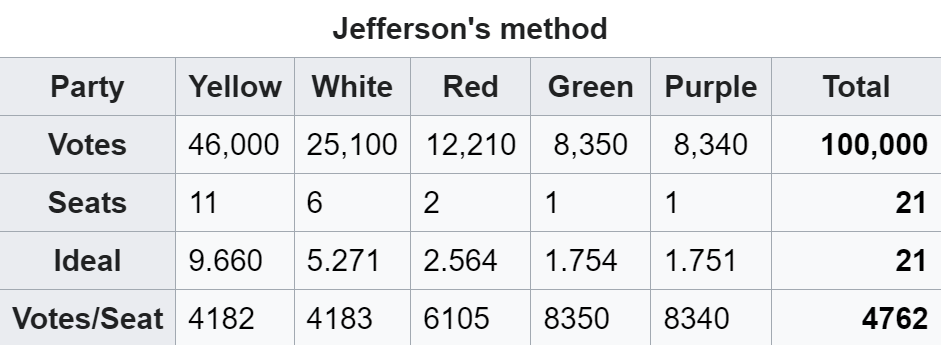
\includegraphics[width=10.41667in,height=\textheight]{images/jefferson.png}
The Yellow Party: has only \(46\%\) of votes, but won
\(11/21\approx 52\%\) majority seats. Violating the
\textbf{Majority-preserving clause}.

\section{Balinski-Young Theorem
(1980)}\label{balinski-young-theorem-1980}

\begin{itemize}
\item
  Any method that follows the quota rule must fail the population
  paradox.
\item
  Any method that is free of the population paradox must fail the quota
  rule for some circumstances.
\item
  Largest remainder method satisfies the quota rule, it violates the
  Alabama paradox and the population paradox.
\item
  The highest averages methods violate the quota rule, avoid population
  paradox and no-show paradox. Not sensitive to spoiler effect. only do
  so (violate quota rule) rarely.
\end{itemize}

\section{Why use geometric mean?}\label{why-use-geometric-mean}

Given two positive numbers \(a\) and \(b\), then the geometric mean of
\(a\) and \(b\) is \[
G=\sqrt{ab}\,.
\] \textbf{AM-GM theorem:} \[
\sqrt{ab}\le \frac{a+b}{2}\,.
\] The equality is true if and if \(a=b\).

\section{GM-equal relative error}\label{gm-equal-relative-error}

\[
a \quad \sqrt{ab} \quad \frac{a+b}{2}\quad b
\] \[
\frac{\sqrt{ab}}{a}=\frac{b}{\sqrt{ab}}\,,
\] that is, the two relative percentage errors are equal: \[
\frac{\sqrt{ab}-a}{a}=\frac{b-\sqrt{ab}}{\sqrt{ab}}\,.
\]

\section{GM-Example}\label{gm-example}

For example, if \(a=2\) and \(b=3\), then
\(\sqrt{2\cdot 3} \approx 2.45\). Therefore, for \(x=2.48\), if
performing geometric rounding, \(2.48\approx 3\). This rounding minimize
the percentage error: \[
\frac{2.48-2}{2}=24\% < \frac{3-2.48}{2.48}\approx 21\% \,.
\]



\end{document}
